\documentclass{ltjsarticle}
\title{パターン認識第8章レポート課題}
\author{201611353 荻野夏樹}
\usepackage{graphicx}
\usepackage{subfiles}
\usepackage{lastpage}
\usepackage{fancyhdr}
\usepackage{amsmath}
\usepackage{amssymb}
\usepackage{ascmac}
\usepackage{url}       % \urlでエスケープなしでurlを表示
\usepackage{listings}  % ソースコード
\usepackage{color}
\usepackage{here}      % figureで[H]を使えるようにする
\usepackage{mathtools} % 参照している式番号のみを表示
\usepackage{bm} % \bm{}でbold,italicでベクトルを表す
\usepackage{titlesec} % sectionの文字サイズを変更
\titleformat*{\section}{\large\bfseries}
\lstset{
	numbers=left,
	numbersep=1em,
%	numberstyle=\tiny\color{red}\noaccsupp,
	frame=single,
%	framesep=\fboxsep,
%	framerule=\fboxrule,
%	rulecolor=\color{red},
%	xleftmargin=\dimexpr\fboxsep+\fboxrule\relax,
%	xrightmargin=\dimexpr\fboxsep+\fboxrule\relax,
	breaklines=true,
	columns=flexible,
	basicstyle=\ttfamily\footnotesize,
	tabsize=4
}
\graphicspath{{../images/}} %実は相対パスで指定してる
%\nonumber
\mathtoolsset{showonlyrefs=true}
\renewcommand{\thesection}{(\arabic{section})}
\renewcommand{\thesubsection}{(\arabic{section}--\arabic{subsection})}

\begin{document}
\maketitle
4つの学習データ
\begin{align*}
	\Bigl\{
		\bigl(t_A=-1,\bm{x}_A=(0,0)^T\bigr),
		\bigl(t_B=-1,\bm{x}_B=(1,0)^T\bigr),
		\bigl(t_C=-1,\bm{x}_C=(0,1)^T\bigr),
		\bigl(t_D=+1,\bm{x}_D=(1,1)^T\bigr)
	\Bigr\}
\end{align*}

\begin{lstlisting}[caption=以降のPythonプログラムが参照する共通の定義部分]
import numpy as np
import matplotlib.pyplot as plt
import math

t_A = -1
x_A = np.array([0,0])
t_B = -1
x_B = np.array([1,0])
t_C = -1
x_C = np.array([0,1])
t_D = 1
x_D = np.array([1,1])
w = np.array([-1,-1])
b = 1.5
\end{lstlisting}

\section{4つの学習データを2次元平面$(x_1 , x_2)$上にクラスラベルを明示してプロットしなさい。}
\begin{figure}[H]
	\centering
	%
	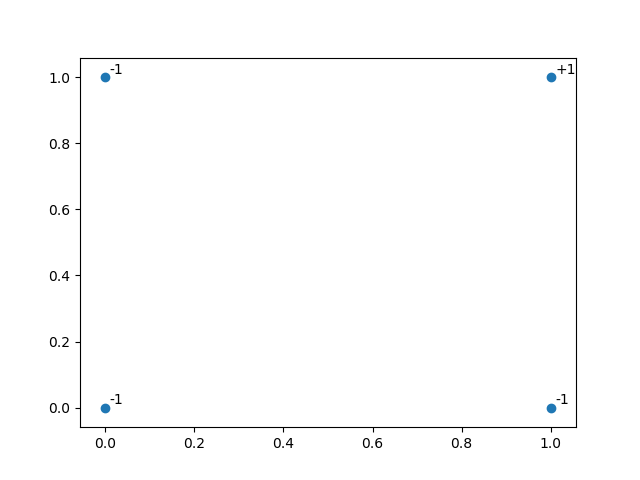
\includegraphics[width=0.5\linewidth]{../images/1_plot_point.png}
	\caption{1\_plot\_point}
	\label{1_plot_point}
\end{figure}
以下のプログラムを用いて作図した。
\begin{lstlisting}
def q1():
    plt.clf()
    plt.scatter(*train_data)
    plt.text(0+0.01 , 0+0.01 , '-1')
    plt.text(1+0.01 , 0+0.01 , '-1')
    plt.text(0+0.01 , 1+0.01 , '-1')
    plt.text(1+0.01 , 1+0.01 , '+1')
    plt.show()
\end{lstlisting}

\section{マージンが最大になる線形識別関数$f(x_1 , x_2)$を視覚的に求め、識別境界を図中に示しなさい。}
図の赤線が求めた識別境界である。
\begin{figure}[H]
	\centering
	%
	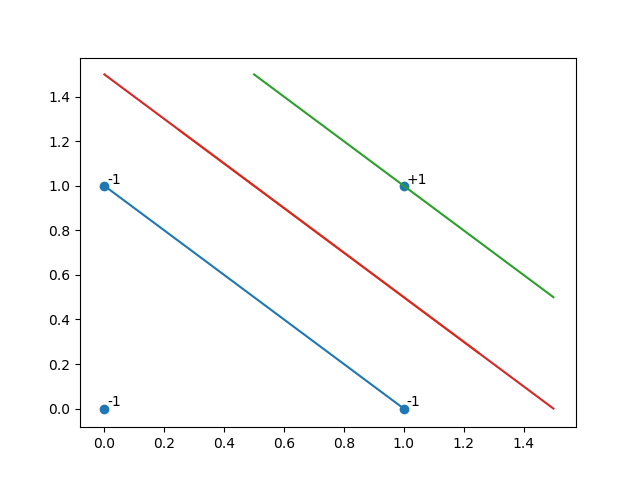
\includegraphics[width=0.5\linewidth]{../images/2_line.png}
	\caption{}
	\label{2_line}
\end{figure}
以下のプログラムを用いて作図した。
\begin{lstlisting}
def q2():
    plt.clf()
    plt.scatter(*train_data)
    plt.text(0+0.01 , 0+0.01 , '-1')
    plt.text(1+0.01 , 0+0.01 , '-1')
    plt.text(0+0.01 , 1+0.01 , '-1')
    plt.text(1+0.01 , 1+0.01 , '+1')
    plt.plot([0+0    , 1+0  ]  , [1+0    , 0+0  ])
    plt.plot([0+0.25 , 1+0.25] , [1+0.25 , 0+0.25])
    plt.plot([0+0.5  , 1+0.5]  , [1+0.5  , 0+0.5])
    plt.plot([0      , 1.5]    , [1.5    , 0])
    plt.show()
\end{lstlisting}


\section{マージンの値はいくつになるか。}
青線と赤線、または緑線と赤線の距離をもとめる。
\begin{align}
	\frac{\sqrt{2}}{4}
\end{align}
となった。

\section{4つの学習データのうち、サポートベクトルはどれか。}
赤線の識別境界との距離が最も近い点を求めればよく、そのような点は$\bm{x}_B,\bm{x}_C,\bm{x}_D$である。

\section{サポートベクトルがKKT条件$ t_i\bigl(w^T x_i + b \bigr) \ge 1 $を満たしているか確認しなさい。満たしていない場合、満たすように識別関数を修正しなさい。}

最初に求めた識別関数は$w = (1,1)^T, b = -1.5$であったが以下のq5を用いて確認したところKKT条件を満たしていなかった。
識別関数を$w = (2,2)^T, b = -3$に2倍に修正したところ、KKT条件を満たすようになった。

\begin{lstlisting}
def KKT(t, x):
    w = 2* np.array([1,1])
    b = 2* -1.5
    return t*(w.transpose() @ x + b)

def q5():
    print(KKT(t_B, x_B)>=1)
    print(KKT(t_C, x_C)>=1)
    print(KKT(t_D, x_D)>=1)
\end{lstlisting}


\section{サポートベクトルのみを用いて双対問題のラグランジュ関数を求めなさい。}

\begin{lstlisting}[caption=Hを求め、Mathematicaの形式に変換するPythonプログラム]
def q6():
    x = [x_B, x_C, x_D]
    t = [t_B, t_C, t_D]
    H = [[t[i]*t[j]*x[i].transpose()@x[j] for j in range(3)]for i in range(3)]
    print(str(H).replace('[','{').replace(']','}'))
    print(t)
\end{lstlisting}
\begin{lstlisting}[caption=output]
{{1, 0, -1}, {0, 1, -1}, {-1, -1, 2}}
[-1, -1, 1]
\end{lstlisting}


ラグランジュ関数は以下のようになった
\begin{align}
	L(\bm{a},\beta) &= \bm{a}^T\bm{1} - \frac{1}{2} \bm{a}^T H\bm{a} - \beta\bm{a}^T t \\
	ただしH &=
	\begin{pmatrix}
		1  & 0  & -1\\
		0  & 1  & -1\\
		-1 & -1 & 2 \\
	\end{pmatrix}
\end{align}

\section{ラグランジュ関数をラグランジュ乗数で微分し、0 とおいて、すべてのラグランジュ乗数の値を求めなさい。}
以下のMathematicaプログラムを用いて求めた。Dは第1引数で指定した式を第2引数で指定した変数で微分した結果を返す関数であり、
Solveは第1引数で指定した方程式を第2引数で指定した変数で解いた結果を返す関数である。
また、Mathematicaでは縦ベクトルと横ベクトルを同一視しているため、内積をとる時に転置しない。
\begin{lstlisting}[caption=input]
H = {{1, 0, -1}, {0, 1, -1}, {-1, -1, 2}};
t = {-1, -1, 1};
L[a0_, a1_, a2_, b_] = a0 + a1 + a2 - 1/2 {a0, a1, a2}.H.{a0, a1, a2} - b*{a0, a1, a2}.t;
Solve[{D[L[a0, a1, a2, b], a0] == 0 &&
       D[L[a0, a1, a2, b], a1] == 0 &&
       D[L[a0, a1, a2, b], a2] == 0 &&
       D[L[a0, a1, a2, b], b ] == 0}, {a0, a1, a2, b}]
\end{lstlisting}
\begin{lstlisting}[caption=output]
{{a0 -> 2, a1 -> 2, a2 -> 4, b -> -3}}
\end{lstlisting}
すなわち、
\begin{align}
	\bm{a} =
	\begin{pmatrix}
		2\\
		2\\
		4
	\end{pmatrix}
	,\ 
	\beta = -3
\end{align}
である。

\section{得られたラグランジュ乗数を用いて最適解$ \bm{w}_0$ を求めなさい。}
\begin{lstlisting}[caption=w\_0を求めるPythonプログラム]
def q8():
    x = [x_B, x_C, x_D]
    t = [t_B, t_C, t_D]
    a = [2,2,4]
    b = -3
    w_0 = sum(a[i]*t[i]*x[i]for i in range(3))
    print(w_0)
\end{lstlisting}
\begin{lstlisting}[caption=output]
[2 2]
\end{lstlisting}
すなわち、
\begin{align}
	\bm{w}_0 =
	\begin{pmatrix}
		2\\
		2\\
	\end{pmatrix}
\end{align}
である。

\section{最適なバイアス $b_0$ を求めなさい。}
\begin{align}
	t_s\bigl(\bm{w}_0^T\bm{x}_s+b_0\bigr)-1&=0を解き\\
	b_0 %= -3
\end{align}

\section{得られた識別関数は、(5)で求めた識別関数と一致したか。}
一致した。
\end{document}
